\documentclass[10pt]{beamer}

%% Based on the original theme by Matthias Vogelgesang

\usetheme[progressbar=frametitle]{metropolis}
\usepackage{appendixnumberbeamer}

\usepackage{booktabs}
\usepackage[scale=2]{ccicons}

\usepackage{pgfplots}
\usepgfplotslibrary{dateplot}

\usepackage{xspace}
\usepackage{xcolor}
\newcommand{\themename}{\textbf{\textsc{metropolis}}\xspace}

%%%%%%%%%%%%%%%%%%%%%%%%%%%%
%% UNCC Theme Adjustments %%
%%%%%%%%%%%%%%%%%%%%%%%%%%%%
\definecolor{CanvasBG}{HTML}{FAFAFA}

% From the official style guide
\definecolor{UnccGreen}{HTML}{00703C}
\definecolor{UnccGold}{HTML}{B3A369}
\definecolor{UnccLightGreen}{HTML}{C3D7A4}
\definecolor{UnccYellow}{HTML}{F0CB00}
\definecolor{UnccOrange}{HTML}{F3901D}
\definecolor{UnccLightYellow}{HTML}{FFF6DC}
\definecolor{UnccBlue}{HTML}{00728F}
\definecolor{UnccPink}{HTML}{DE3A6E}
\definecolor{White}{HTML}{FFFFFF}
\definecolor{LightGray}{HTML}{DDDDDD}

% Supporting Color Palette
\definecolor{WarmGray}{HTML}{696158}
\definecolor{StoneGray}{HTML}{717C7D}
\definecolor{DarkGreen}{HTML}{2C5234}
\definecolor{LightGreen}{HTML}{509E2F}
\definecolor{BrightGold}{HTML}{F0CB00}

% Screamers
\definecolor{Royal}{HTML}{72246C}
\definecolor{Ocean}{HTML}{006BA6}
\definecolor{Flash}{HTML}{B52555}
\definecolor{Citrus}{HTML}{FFB81C}
\definecolor{Spring}{HTML}{CEDC00}

% Serenity
\definecolor{Garden}{HTML}{B7CE95}
\definecolor{Sand}{HTML}{F0E991}
\definecolor{Bloom}{HTML}{F1E6B2}
\definecolor{Clay}{HTML}{B7B09C}
\definecolor{Cloud}{HTML}{BAC5B9}

% Set colors here
\setbeamercolor{frametitle}{bg=UnccGreen}
\setbeamercolor{progress bar}{bg=BrightGold, fg=UnccGreen}
\setbeamercolor{alerted text}{fg=Flash}

\setbeamercolor{block title}{bg=LightGreen, fg=White}
\setbeamercolor{block title example}{bg=Ocean, fg=White}
\setbeamercolor{block title alerted}{bg=Citrus, fg=White}
\setbeamercolor{block body}{bg=CanvasBG}

\metroset{titleformat=smallcaps, progressbar=foot, sectionpage=none}

\makeatletter
\setlength{\metropolis@progressinheadfoot@linewidth}{2pt}
\setlength{\metropolis@titleseparator@linewidth}{2pt}
\setlength{\metropolis@progressonsectionpage@linewidth}{2pt}
%%%%%%%%%%%%%%%%%%%%%%%%%%%%
%% UNCC Theme Adjustments %%
%%%%%%%%%%%%%%%%%%%%%%%%%%%%


\title{Antrittsvortrag}
\subtitle{Sensorbasierter Orientierungssinn\\mit künstlichen neuronalen Netzen\\und Entscheidungsbäumen}
% \date{\today}
\date{21.04.2021}
\author{Tom Dymel}
\institute{Masterarbeit\\Technische Universität Hamburg}
% \titlegraphic{\hfill\includegraphics[height=1.5cm]{logo.pdf}}

\begin{document}

\maketitle

\section{Motivation}
\begin{frame}{Motivation}
\begin{itemize}
    \item Orientierungssinn von Tieren und Menschen
    \item Indoor-Lokalisierung hohe Infrastrukturkosten
    \item Mian untersuchte FFNN und simulierte Daten
    \item Entscheidungsbäume potentiell effizienter
\end{itemize}
\end{frame}

\section{Ziele}
\begin{frame}{Ziele}
\begin{itemize}
    \item Diskrete Orte oder Wege erkennen können
    \item Robustheit gegenüber Fehler/Anomalien
    \item Trainings- und Testdaten simulativ erfassen
    \item Geeignete Features wählen
    \item Berücksichtigung von Batterielaufzeit und Limitierung des $\mu C$
    \item Vergleich von KNN und Entscheidungsbaum
\end{itemize}
\end{frame}

\section{Mögliche Sensoren}
\begin{frame}{Mögliche Sensoren}
\begin{itemize}
    \item Beschleunigung
    \item Gyroskop
    \item Licht
    \color{red}
    \item Magnetfeld
    \item Temperatur
    \item Geräusche
    \item WLAN Access-Points
\end{itemize}
\end{frame}

\begin{frame}{Diskrete Orte unterscheiden}
    \begin{figure}
        \centering
        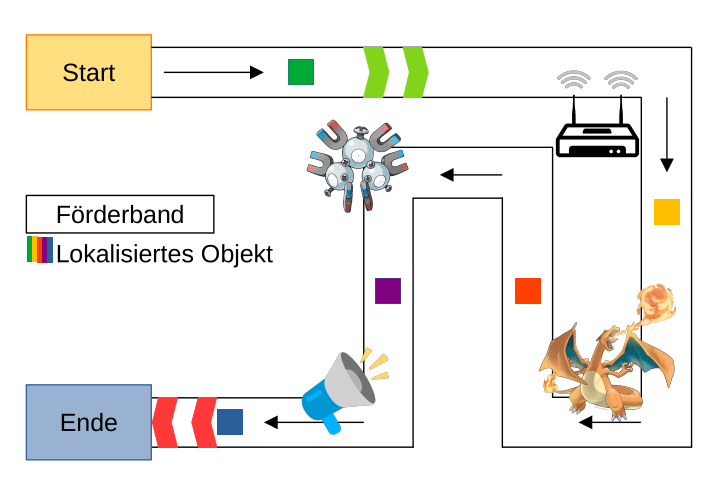
\includegraphics[width=\linewidth]{setting_complex.png}
    \end{figure}
\end{frame}

\section{Trainings- und Testdaten}
\begin{frame}{Trainings- und Testdaten}
\begin{itemize}
    \item Simulation von Routen durch CoppeliaSim
    \begin{itemize}
        \item Realistische Physik-Engine
        \item Förderband System
        \item Beschleunigungs-, Lichtsensor und Gyroskop
    \end{itemize}
    \item Post-Processing
    \begin{itemize}
        \item Feature-Extrahierung
        \color{red}
        \item Ergänzung von Sensoren
        \item Fault-Injection
        \item Synthetische Routen
        \item Filterung basierend auf künstliche Interrupts
    \end{itemize}
\end{itemize}
\end{frame}

\section{Entscheidungsbaum und KNN}
\begin{frame}{Modell}
    \begin{figure}
        \centering
        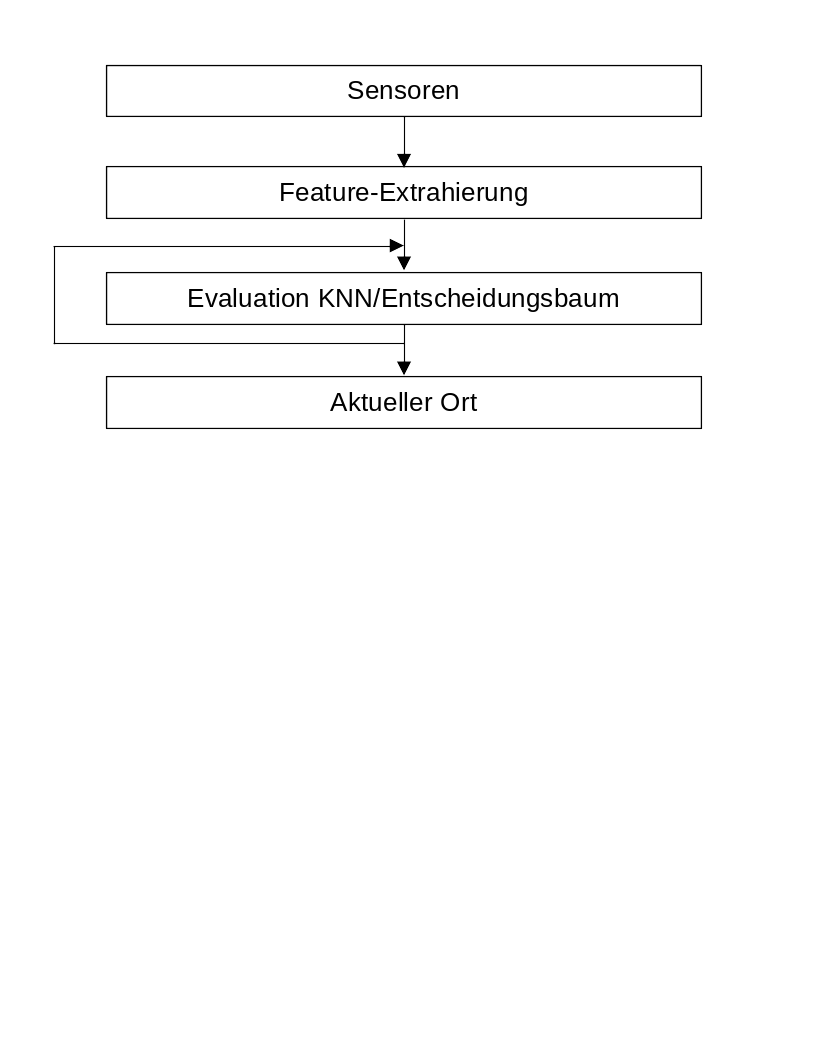
\includegraphics[width=\linewidth]{modell.png}
    \end{figure}
\end{frame}

\section{Zeitplan}
\begin{frame}{Zeitplan}
\begin{figure}
    \centering
    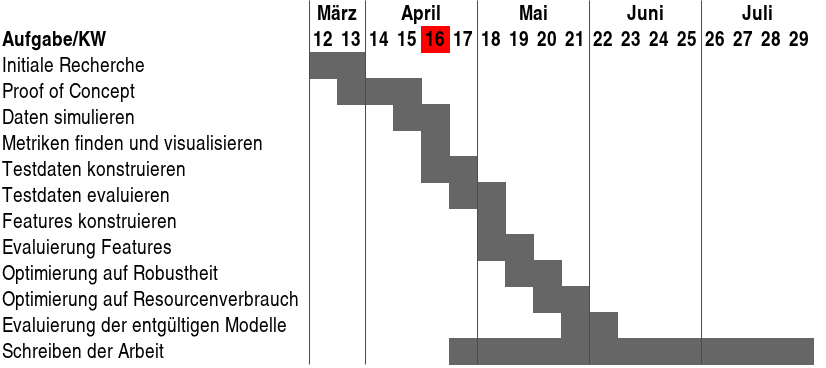
\includegraphics[width=\linewidth]{Projektplan.png}
\end{figure}
\end{frame}
\begin{frame}[standout]
  Fragen?
\end{frame}

\begin{frame}{Route: "Many Corners"}
    \begin{figure}
        \centering
        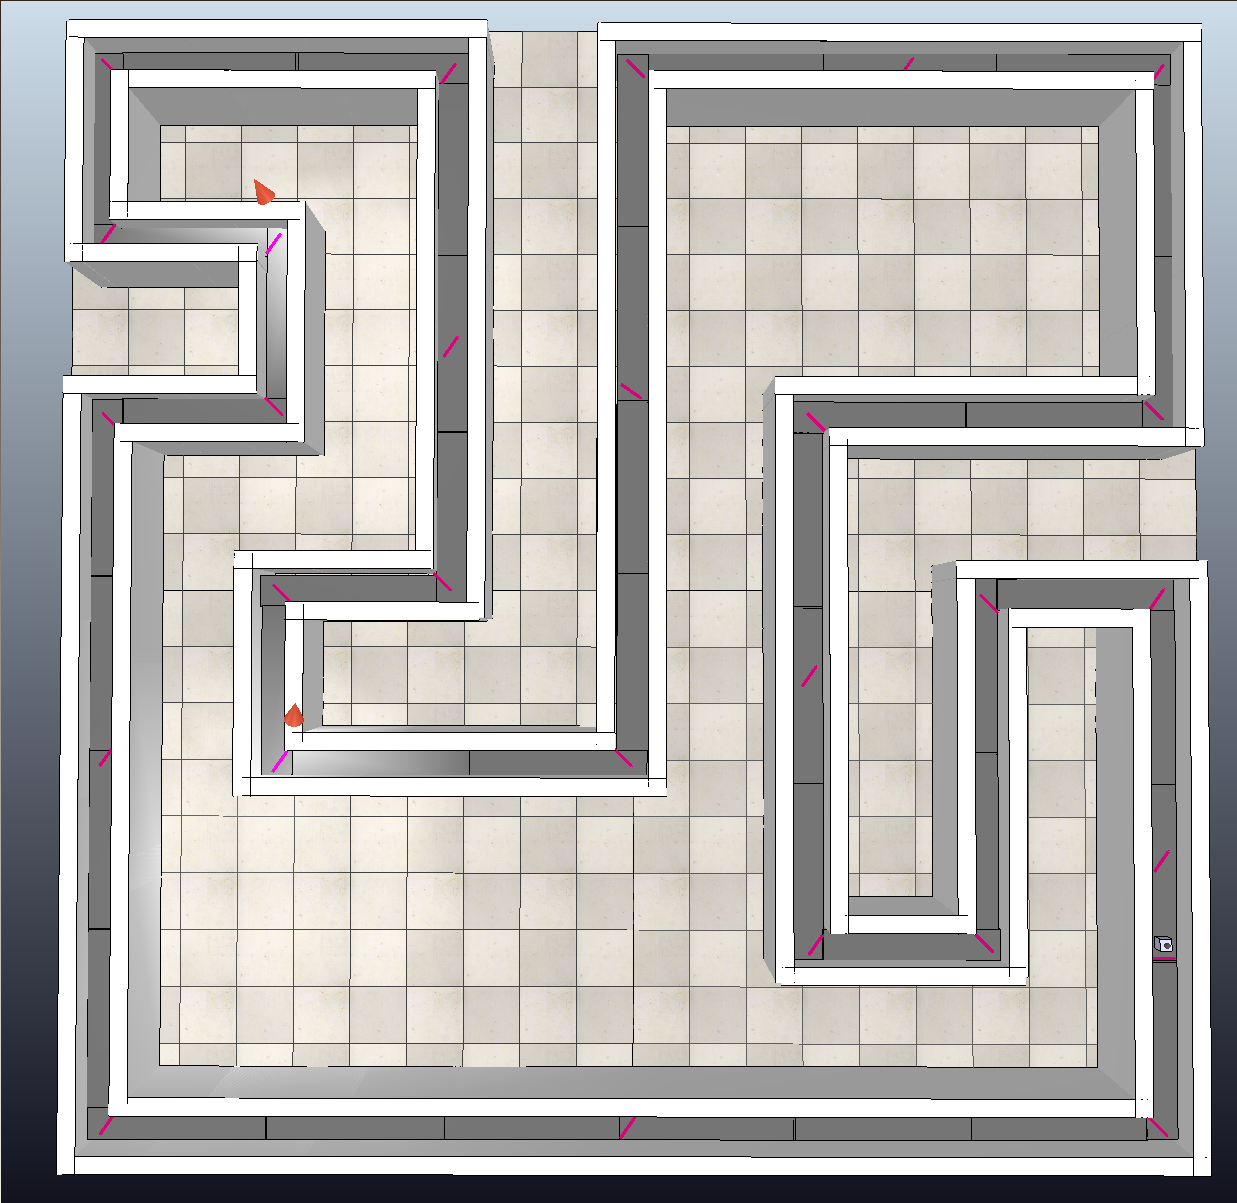
\includegraphics[width=0.8\linewidth]{many_corners.png}
    \end{figure}
\end{frame}

\begin{frame}{Route: "Simple Square"}
    \begin{figure}
        \centering
        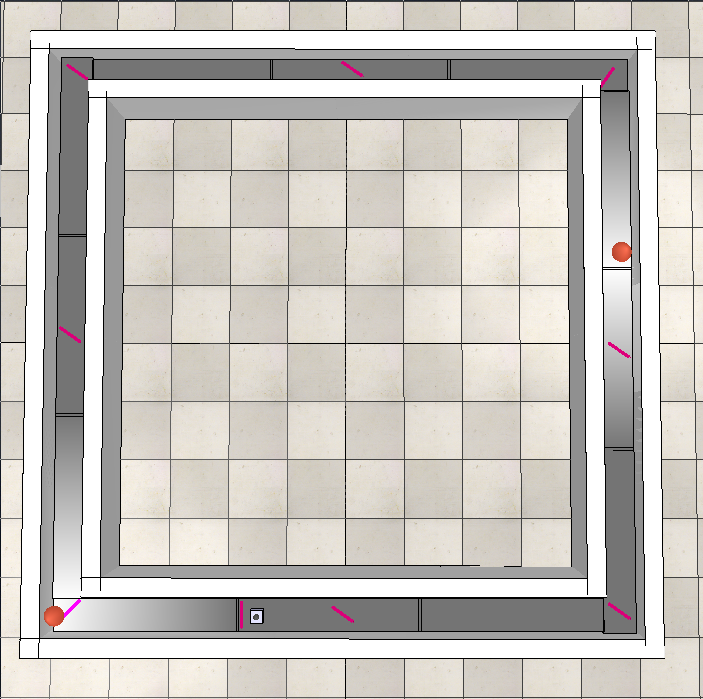
\includegraphics[width=0.8\linewidth]{simple_square.png}
    \end{figure}
\end{frame}

\begin{frame}{Route: "Long Rectangle"}
    \begin{figure}
        \centering
        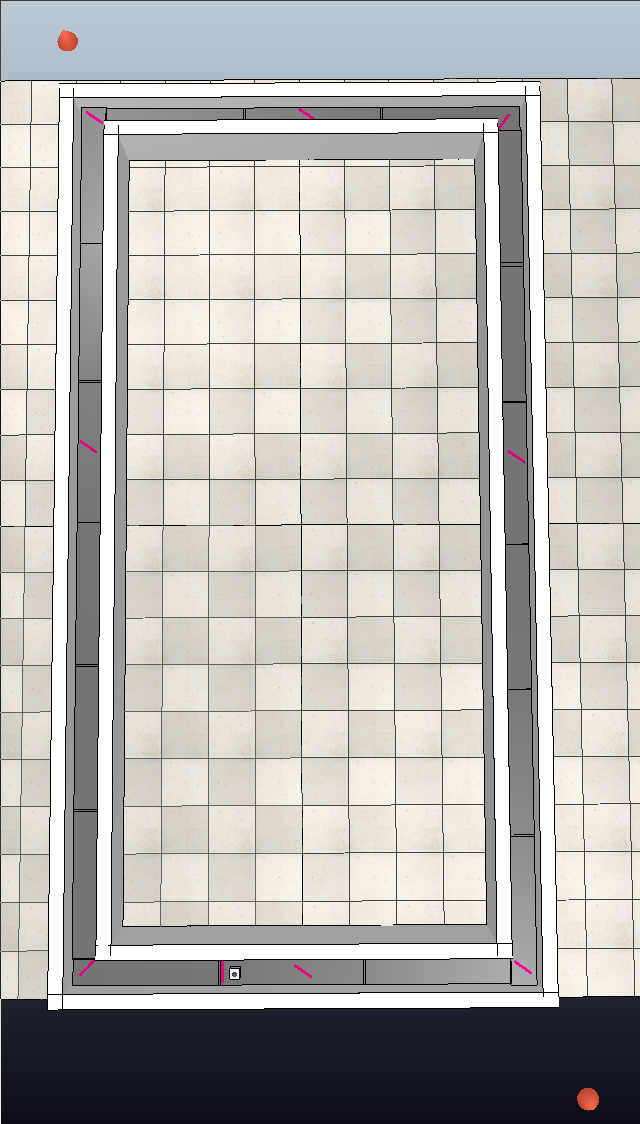
\includegraphics[angle=90,width=\linewidth]{long_rectangle.png}
    \end{figure}
\end{frame}

\begin{frame}{Route: "Rectangle with Ramp"}
    \begin{figure}
        \centering
        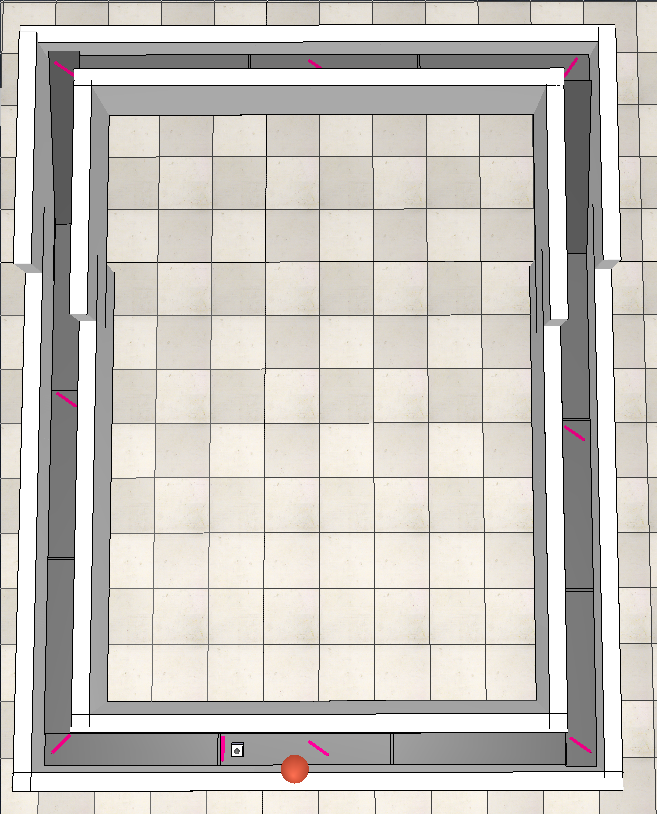
\includegraphics[angle=90,width=0.9\linewidth]{rectangle_with_ramp.png}
    \end{figure}
\end{frame}

\end{document}

